\chapter[APÊNDICE \ref{Ap:cylinder}]{Escoamento sobre um cilindro}
\label{Ap:cylinder}

Para o seguinte problema considerou-se um cilindro circular de raio $R=0,5$ em um domínio retangular $\Omega=[0,112R]\times[0,100R]$, sendo o centro do cilindro posicionado sobre o ponto $(36,50)R$. As condições de contorno consideradas foram de entrada na face esquerda ($x_1=0$) do domínio ($\BB{u}=\{u_\infty,0\}^T$), condição de velocidade vertical nula nas faces inferior e superior ($u_2=0$ em $x_2=0$ e $x_2=100R$) e pressão nula no ponto $(112,100)R$. Como condição inicial aplicou-se uma velocidade $\BB{u}=\{u_\infty,0\}^T$ em todo o domínio. A densidade do fluido foi de $\rho=1$ com viscosidade $\nu=0,01$ e uma velocidade $u_\infty=1$, que, ao considerar o comprimento característico como o diâmetro do cilindro, obtém-se $\Rey=100$.

Para a simulação numérica considerou-se a malha apresentada na Figura \ref{fig:cyl-mesh}, a qual possui 4656 elementos finitos. Assim, estudou-se o escoamento em situação onde não se aplicou nenhum modelo de turbulência, seguido da aplicação dos modelos LES e VMS. Todas as simulações foram conduzidas utilizando os elementos de aproximação linear, quadrática e Taylor-Hood P2P1. Para os elementos linear e quadrático aplicou-se em todos os casos o estabilizador PSPG para obtenção de resultados consistentes. O problema discretizado possui 7263 graus de liberdade para elemento linear, 28494 para elemento quadrático e 21417 para P2P1. O intervalo de tempo foi de $t\in[0,200]$ com passos de $\Delta t=0,1$.

\begin{figure}[h!]
    \centering
    \caption{Malha utilizada para a simulação de escoamento sobre um cilindro.}
    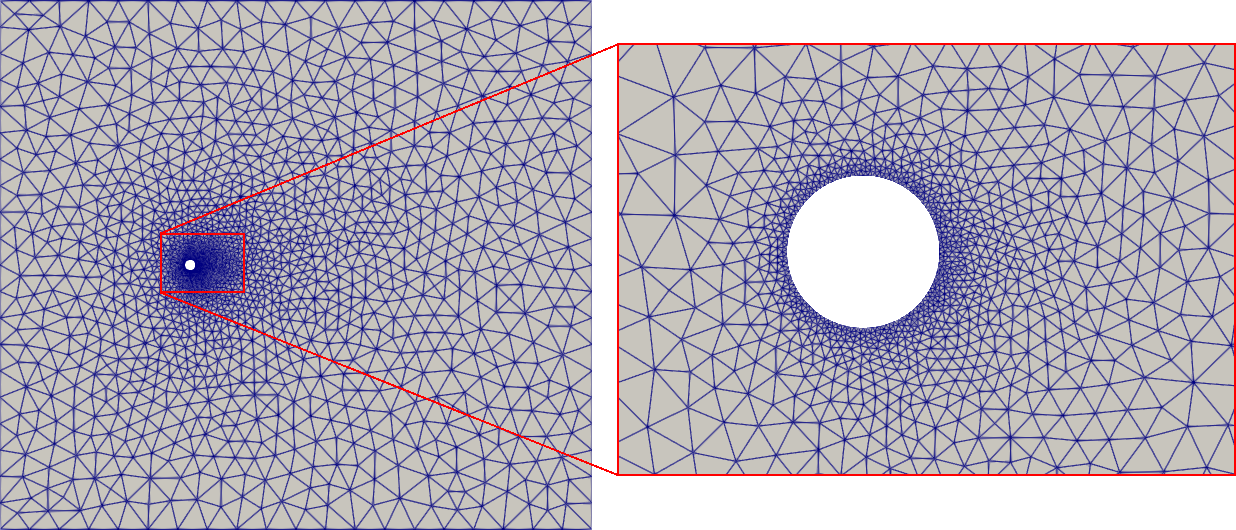
\includegraphics[width=\linewidth]{Figuras/cylinder/analise2/mesh.png}
    \\Fonte: Autoria Própria (\the\year).
    \label{fig:cyl-mesh}
\end{figure}

Para análise dos resultados determinou-se os coeficientes de arrasto (\textit{Drag} - $C_D$) e de sustentação (\textit{Lift} - $C_L$), dados respectivamente por:

\begin{subequations}
    \begin{equation}
        C_D=\frac{2F_D}{\rho\norm{\BB{u}_\infty}^2L}\text{ e}
    \end{equation}
    \begin{equation}
        C_L=\frac{2F_L}{\rho\norm{\BB{u}_\infty}^2L}\text{,}
    \end{equation}
\end{subequations}

\noindent em que $F_D$ e $F_L$ são as forças de arrasto e de sustentação, calculados como:

\begin{subequations}
    \begin{equation}
        F_D=\int_{\Gamma_S}{\sigma_{1j}n_jd\Gamma_S}\text{ e}
    \end{equation}
    \begin{equation}
        F_L=\int_{\Gamma_S}{\sigma_{2j}n_jd\Gamma_S}\text{,}
    \end{equation}
\end{subequations}

\noindent sendo $\Gamma_S$ a fronteira do cilindro e $\BB{n}$ o vetor normal à $\Gamma_S$.

Outro parâmetro possível de se verificar é o número de Strouhal ($\Str$), que se trata de um número adimensional que busca relacionar a frequência de oscilação devido à formação de vórtices e a velocidade do fluido. Esse parâmetro pode ser determinado por:

\begin{equation}
    \Str=\frac{f_vL}{\norm{\BB{u}_\infty}}\text{,}
\end{equation}

\noindent sendo $f_v$ a frequência de desprendimento de vórtices.

As Figuras \ref{fig:cyl-draglift-None}, \ref{fig:cyl-draglift-LES} e \ref{fig:cyl-draglift-VMS} apresentam os coeficientes de arrasto e de sustentação obtidos em todas as simulações. Os campos de velocidades e de pressões atuantes no cilindro no instante $t=120$ são apresentados nas Figuras \ref{fig:vel-pre-Lin}, \ref{fig:vel-pre-Qua} e \ref{fig:vel-pre-TH}.

\begin{figure}[h!]
    \centering
    \caption{Valores ao longo do tempo na simulação sem modelo de:}
    \begin{subfigure}{.49\textwidth}
        \centering
        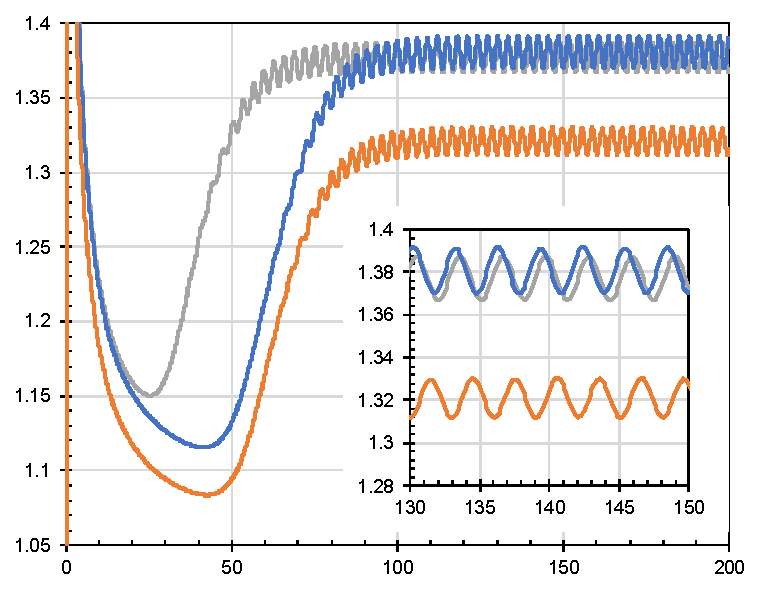
\includegraphics[width=\linewidth]{Figuras/cylinder/analise2/none-drag.pdf}
        \caption{coeficiente de arrasto.}
    \end{subfigure}
    \begin{subfigure}{.49\textwidth}
        \centering
        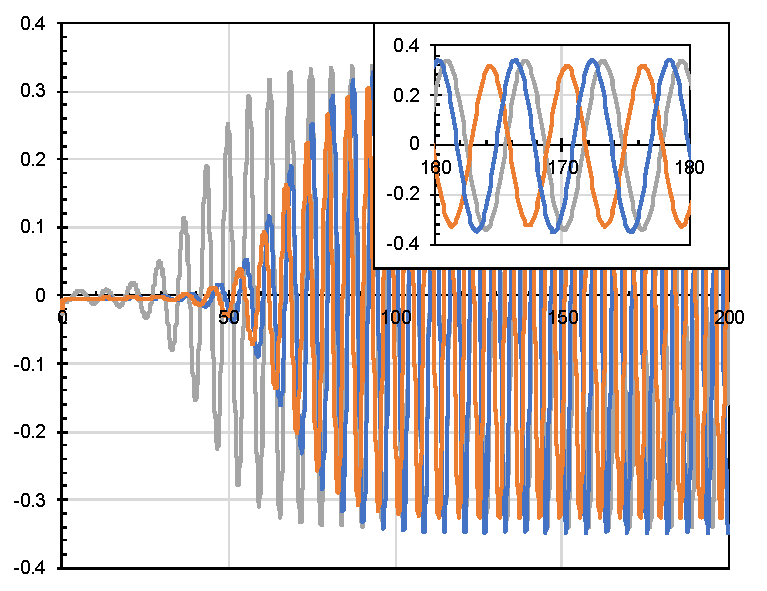
\includegraphics[width=\linewidth]{Figuras/cylinder/analise2/none-lift.pdf}
        \caption{coeficiente de sustentação.}
    \end{subfigure}
    \begin{subfigure}{\textwidth}
        \centering
        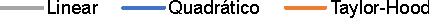
\includegraphics[width=.4\linewidth]{Figuras/cylinder/analise2/legenda.pdf}
    \end{subfigure}
    \\Fonte: Autoria Própria (\the\year).
    \label{fig:cyl-draglift-None}
\end{figure}

\begin{figure}[h!]
    \centering
    \caption{Valores ao longo do tempo na simulação LES de:}
    \begin{subfigure}{.49\textwidth}
        \centering
        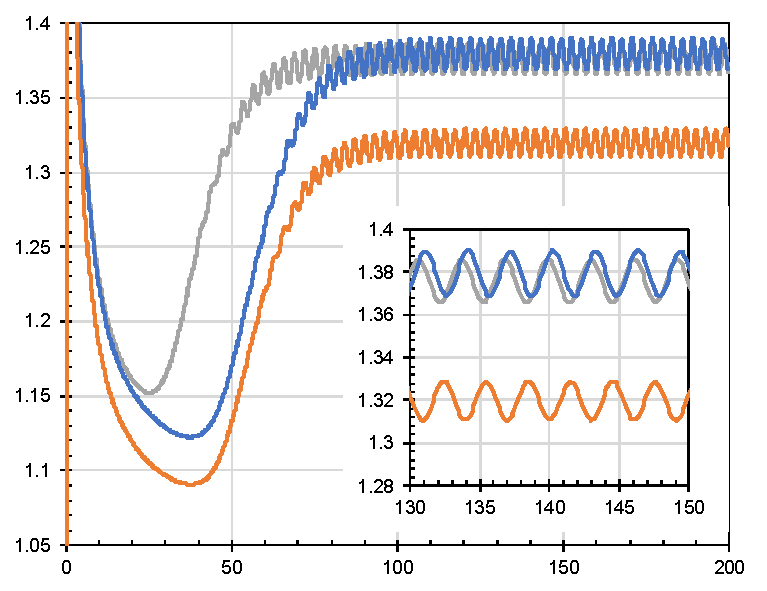
\includegraphics[width=\linewidth]{Figuras/cylinder/analise2/LES-drag.pdf}
        \caption{coeficiente de arrasto.}
    \end{subfigure}
    \begin{subfigure}{.49\textwidth}
        \centering
        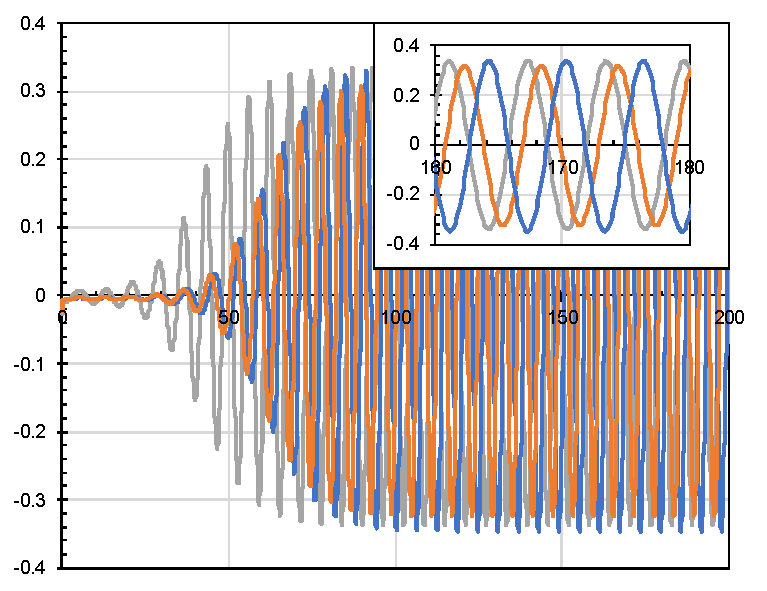
\includegraphics[width=\linewidth]{Figuras/cylinder/analise2/LES-lift.pdf}
        \caption{coeficiente de sustentação.}
    \end{subfigure}
    \begin{subfigure}{\textwidth}
        \centering
        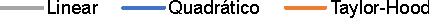
\includegraphics[width=.4\linewidth]{Figuras/cylinder/analise2/legenda.pdf}
    \end{subfigure}
    \\Fonte: Autoria Própria (\the\year).
    \label{fig:cyl-draglift-LES}
\end{figure}

\begin{figure}[h!]
    \centering
    \caption{Valores ao longo do tempo na simulação VMS de:}
    \begin{subfigure}{.49\textwidth}
        \centering
        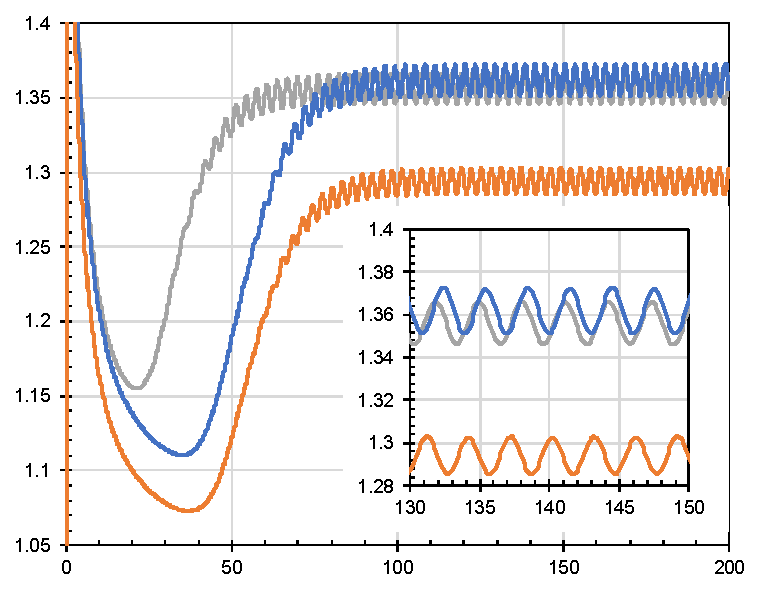
\includegraphics[width=\linewidth]{Figuras/cylinder/analise2/VMS-drag.pdf}
        \caption{coeficiente de arrasto.}
    \end{subfigure}
    \begin{subfigure}{.49\textwidth}
        \centering
        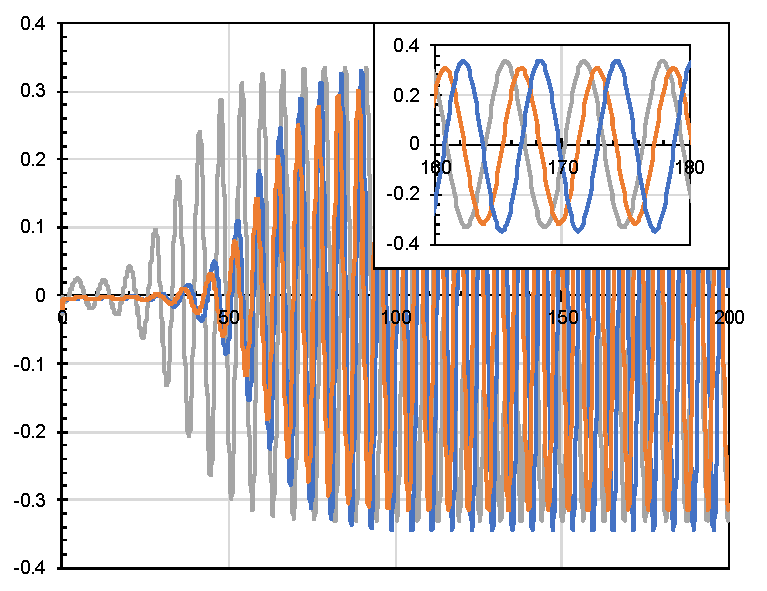
\includegraphics[width=\linewidth]{Figuras/cylinder/analise2/VMS-lift.pdf}
        \caption{coeficiente de sustentação.}
    \end{subfigure}
    \begin{subfigure}{\textwidth}
        \centering
        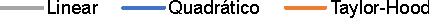
\includegraphics[width=.4\linewidth]{Figuras/cylinder/analise2/legenda.pdf}
    \end{subfigure}
    \\Fonte: Autoria Própria (\the\year).
    \label{fig:cyl-draglift-VMS}
\end{figure}

Os valores da média e da amplitude dos coeficientes de arrasto e de sustentação após o escoamento atingir o equilíbrio dinâmico, assim como o número de Strouhal, são apresentados na Tabela \ref{tab:cyl-res}.

\begin{table}[h!]
    \centering
    \newcommand{\celc}{\multicolumn{1}{c}}
    \newcommand{\ccelc}{\multicolumn{2}{c}}
    \caption{Valores das propriedades dos coeficientes de arrasto e de sustentação para os modelos analisados.}
    \begin{tabular}{llllllll}
        \hline
        \MR{2}{*}{Param.}    & \celc{\MR{2}{*}{Modelo}} & \ccelc{Linear} & \ccelc{Quadrático} & \ccelc{Taylor-Hood}                                           \\\cline{3-8}
                             & \celc{}                  & \celc{Drag}    & \celc{Lift}        & \celc{Drag}         & \celc{Lift} & \celc{Drag} & \celc{Lift} \\\hline
        \MR{3}{*}{Amplitude} & Nenhum                   & 0,0102         & 0,3383             & 0,0109              & 0,3436      & 0,0094      & 0,3219      \\
                             & VMS                      & 0,0101         & 0,3333             & 0,0108              & 0,3411      & 0,0088      & 0,3114      \\
                             & LES                      & 0,0101         & 0,3365             & 0,0107              & 0,3417      & 0,0092      & 0,3200      \\\hline
        \MR{3}{*}{Média}     & Nenhum                   & 1,3772         & -0,0006            & 1,3808              & -0,0080     & 1,3209      & -0,0032     \\
                             & VMS                      & 1,3561         & 0,0046             & 1,3620              & -0,0007     & 1,2939      & -0,0083     \\
                             & LES                      & 1,3760         & -0,0003            & 1,3794              & -0,0031     & 1,3199      & -0,0007     \\\hline
        \MR{3}{*}{Strouhal}  & Nenhum                   & \ccelc{0,1594} & \ccelc{0,1623}     & \ccelc{0,1627}                                                \\
                             & VMS                      & \ccelc{0,1588} & \ccelc{0,1634}     & \ccelc{0,1649}                                                \\
                             & LES                      & \ccelc{0,1590} & \ccelc{0,1614}     & \ccelc{0,1629}                                                \\\hline
    \end{tabular}
    \\Fonte: Autoria Própria (\the\year).
    \label{tab:cyl-res}
\end{table}

Comparando-se os números de Strouhal calculados com aqueles obtidos por \citeonline{fernandes2020tecnica}, que obteve, para a mesma geometria de domínio e mesmas condições de contorno, um $\Str=0,165$ e amplitude do coeficiente de sustentação de 0,3422, \citeonline{tezduyar1992incompressible}, os quais verificaram $\Str$ entre 0,166 e 0,170, \citeonline{najafi2012meshless}, com valor de 0,182, e \citeonline{codina2006numerical}, com velores entre 0,177 e 0,184. As variações observadas entre os números de Strouhal dos diferentes autores podem ser devidas às diferenças nas dimensões dos domínios utilizados, assim como as diferentes condições de contorno aplicadas por cada um. No entanto ainda observa-se que em todos os casos os valores calculados nas simulações ainda são bem próximos. Já com relação à amplitude do coeficiente de sustentação, observa-se que as simulações utilizando elementos quadráticos obtiveram melhor concordância com a obtida por \citeonline{fernandes2020tecnica}. A mínima diferença observada entre os parâmetros calculados em uma simulação sem aplicação de modelo e aquelas que aplicam os modelos VMS e LES, deve-se ao fato do número de Reynolds ser muito baixo, pois, como apontado por \citeonline{fernandes2020tecnica}, esse tipo de escoamento (com $\Rey$ entre 50 e 200) apresenta a formação de vórtices laminares, denominada de esteira de Von Kárman. Para uma verificação mais precisa dessa influência, deve-se partir para uma análise tridimensional com número de Reynolds superiores à 200. Em termos de comparação entre os diferentes tipos de aproximação, verifica-se que tanto os elementos lineares e quadráticos atingiram um regime permanente próximos, enquanto o elemento P2P1 apresentou um amortecimento excessivo, tanto no coeficiente de arrasto, quanto no de sustentação. Já realizando uma comparação dos modelos entre si, verifica-se que em todos os casos o coeficiente de sustentação se manteve inalterado, enquanto o coeficiente de arrasto resultou em uma média menor em relação à simulação LES e sem modelo, porém, mantendo os demais parâmetros muito próximos.

%Vale observar ainda que a simulação VMS linear apresentou um amortecimento menor em relação ao início das oscilações, porém converge para valores muito próximos ao quadrático ao longo do tempo. Já a simulação LES inicia sua oscilação próxima ao VMS quadrático, entretanto com uma média de oscilação menor que a do VMS, em especial ao se observar o coeficiente de arrasto. Tal efeito pode ser devido ao relatado por \citeonline{germano1991dynamic,hughes2000large}, que apontam a ocorrência de um amortecimento excessivo provocado pelo tensor SGS de Smagorinsky.

\begin{figure}[h!]
    \centering
    \caption{Campos de velocidades e de pressões no instante $t=120$ para elemento de aproximação linear.}
    \begin{subfigure}{\textwidth}
        \begin{subfigure}{\textwidth}\centering
            \begin{subfigure}{.42\textwidth}
                \caption*{Campo de velocidades.}
                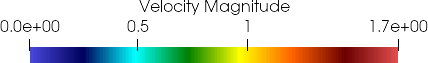
\includegraphics[width=\linewidth]{Figuras/cylinder/analise2/lu.png}
            \end{subfigure}
            \begin{subfigure}{.42\textwidth}
                \caption*{Campo de pressões.}
                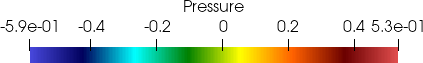
\includegraphics[width=\linewidth]{Figuras/cylinder/analise2/lp.png}
            \end{subfigure}
        \end{subfigure}
    \end{subfigure}
    \begin{subfigure}{\textwidth}\centering
        \begin{subfigure}{.49\textwidth}
            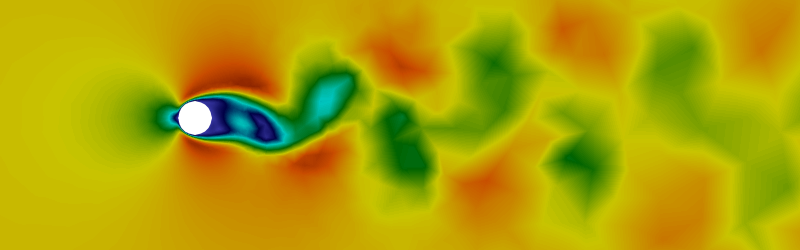
\includegraphics[width=\linewidth]{Figuras/cylinder/analise2/none-Lin-u.png}
        \end{subfigure}
        \begin{subfigure}{.49\textwidth}
            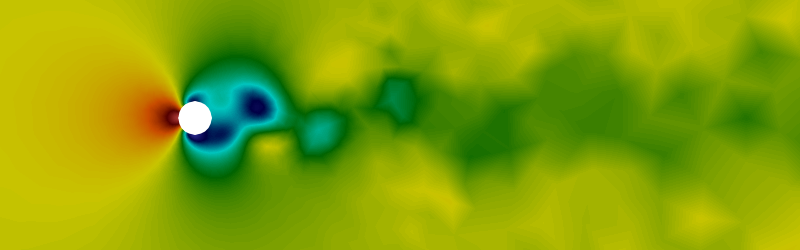
\includegraphics[width=\linewidth]{Figuras/cylinder/analise2/none-Lin-p.png}
        \end{subfigure}
        \caption{Sem modelo}
    \end{subfigure}
    \begin{subfigure}{\textwidth}\centering
        \begin{subfigure}{.49\textwidth}
            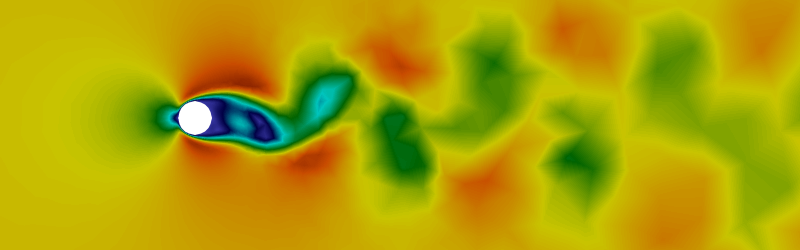
\includegraphics[width=\linewidth]{Figuras/cylinder/analise2/LES-Lin-u.png}
        \end{subfigure}
        \begin{subfigure}{.49\textwidth}
            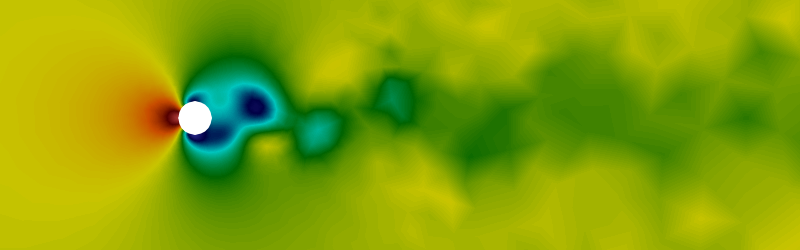
\includegraphics[width=\linewidth]{Figuras/cylinder/analise2/LES-Lin-p.png}
        \end{subfigure}
        \caption{LES}
    \end{subfigure}
    \begin{subfigure}{\textwidth}\centering
        \begin{subfigure}{.49\textwidth}
            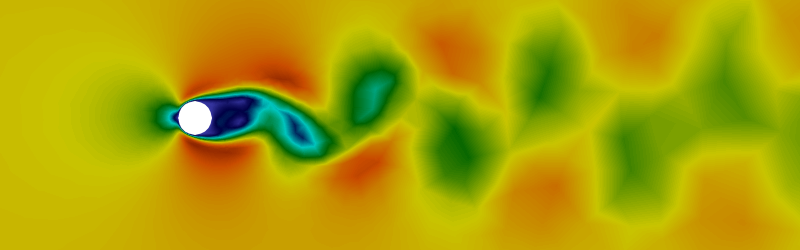
\includegraphics[width=\linewidth]{Figuras/cylinder/analise2/VMS-Lin-u.png}
        \end{subfigure}
        \begin{subfigure}{.49\textwidth}
            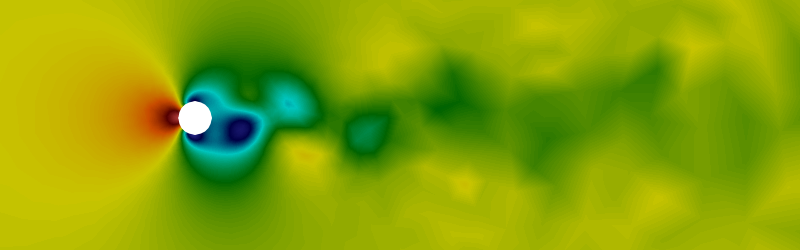
\includegraphics[width=\linewidth]{Figuras/cylinder/analise2/VMS-Lin-p.png}
        \end{subfigure}
        \caption{VMS}
    \end{subfigure}
    \\Fonte: Autoria Própria (\the\year).
    \label{fig:vel-pre-Lin}
\end{figure}

\begin{figure}[h!]
    \centering
    \caption{Campos de velocidades e de pressões no instante $t=120$ para elemento de aproximação quadrática.}
    \begin{subfigure}{\textwidth}
        \begin{subfigure}{\textwidth}\centering
            \begin{subfigure}{.42\textwidth}
                \caption*{Campo de velocidades.}
                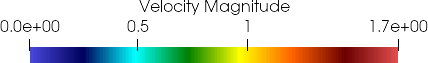
\includegraphics[width=\linewidth]{Figuras/cylinder/analise2/lu.png}
            \end{subfigure}
            \begin{subfigure}{.42\textwidth}
                \caption*{Campo de pressões.}
                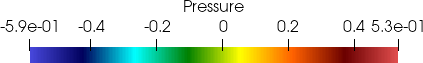
\includegraphics[width=\linewidth]{Figuras/cylinder/analise2/lp.png}
            \end{subfigure}
        \end{subfigure}
    \end{subfigure}
    \begin{subfigure}{\textwidth}\centering
        \begin{subfigure}{.49\textwidth}
            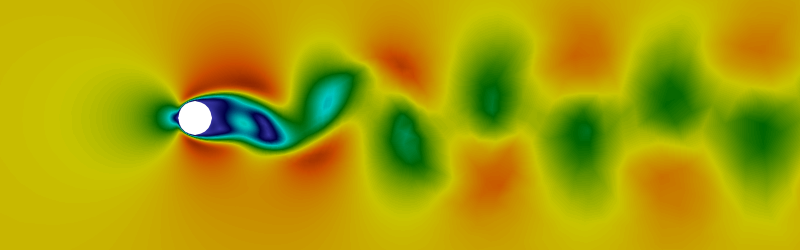
\includegraphics[width=\linewidth]{Figuras/cylinder/analise2/none-Qua-u.png}
        \end{subfigure}
        \begin{subfigure}{.49\textwidth}
            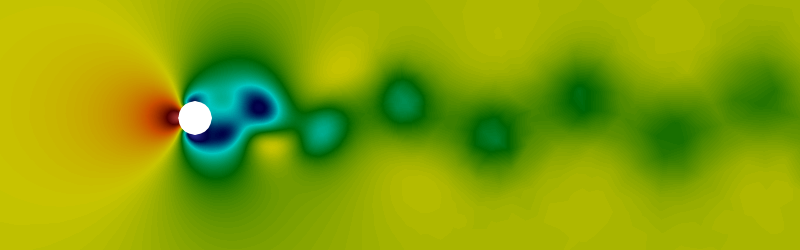
\includegraphics[width=\linewidth]{Figuras/cylinder/analise2/none-Qua-p.png}
        \end{subfigure}
        \caption{Sem modelo}
    \end{subfigure}
    \begin{subfigure}{\textwidth}\centering
        \begin{subfigure}{.49\textwidth}
            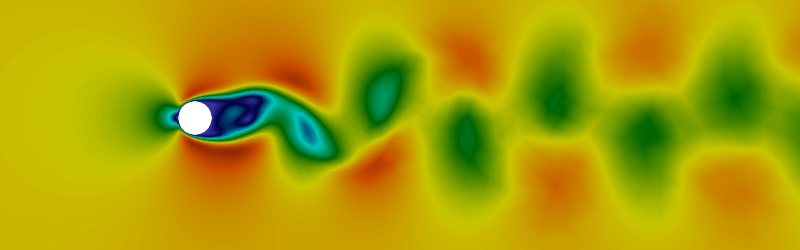
\includegraphics[width=\linewidth]{Figuras/cylinder/analise2/LES-Qua-u.png}
        \end{subfigure}
        \begin{subfigure}{.49\textwidth}
            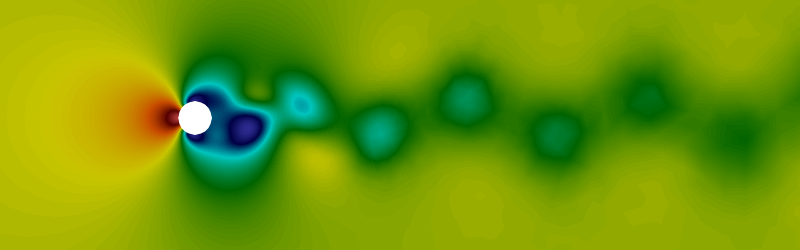
\includegraphics[width=\linewidth]{Figuras/cylinder/analise2/LES-Qua-p.png}
        \end{subfigure}
        \caption{LES}
    \end{subfigure}
    \begin{subfigure}{\textwidth}\centering
        \begin{subfigure}{.49\textwidth}
            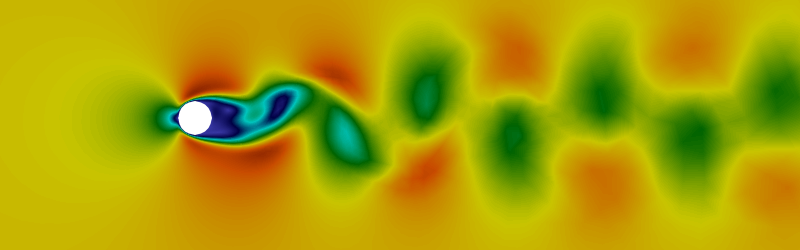
\includegraphics[width=\linewidth]{Figuras/cylinder/analise2/VMS-Qua-u.png}
        \end{subfigure}
        \begin{subfigure}{.49\textwidth}
            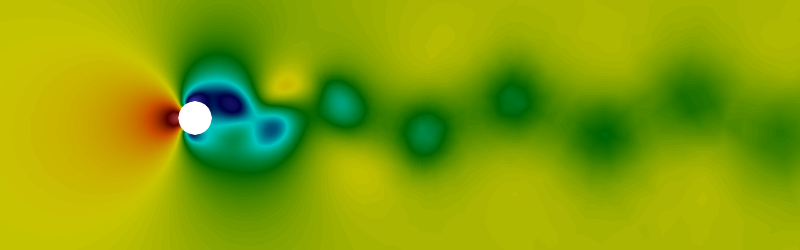
\includegraphics[width=\linewidth]{Figuras/cylinder/analise2/VMS-Qua-p.png}
        \end{subfigure}
        \caption{VMS}
    \end{subfigure}
    \\Fonte: Autoria Própria (\the\year).
    \label{fig:vel-pre-Qua}
\end{figure}

\begin{figure}[h!]
    \centering
    \caption{Campos de velocidades e de pressões no instante $t=120$ para elemento Taylor-Hood P2P1.}
    \begin{subfigure}{\textwidth}
        \begin{subfigure}{\textwidth}\centering
            \begin{subfigure}{.42\textwidth}
                \caption*{Campo de velocidades.}
                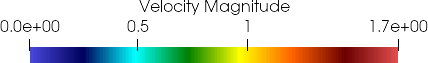
\includegraphics[width=\linewidth]{Figuras/cylinder/analise2/lu.png}
            \end{subfigure}
            \begin{subfigure}{.42\textwidth}
                \caption*{Campo de pressões.}
                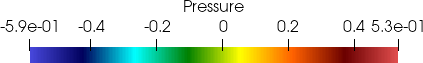
\includegraphics[width=\linewidth]{Figuras/cylinder/analise2/lp.png}
            \end{subfigure}
        \end{subfigure}
    \end{subfigure}
    \begin{subfigure}{\textwidth}\centering
        \begin{subfigure}{.49\textwidth}
            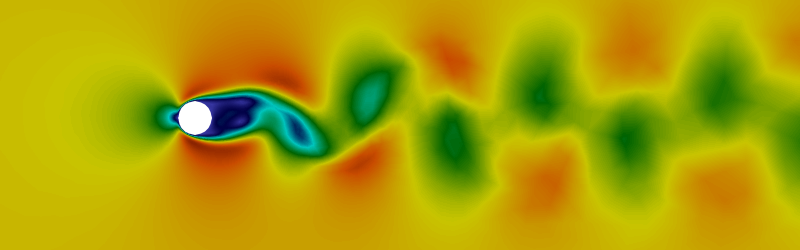
\includegraphics[width=\linewidth]{Figuras/cylinder/analise2/none-TH-u.png}
        \end{subfigure}
        \begin{subfigure}{.49\textwidth}
            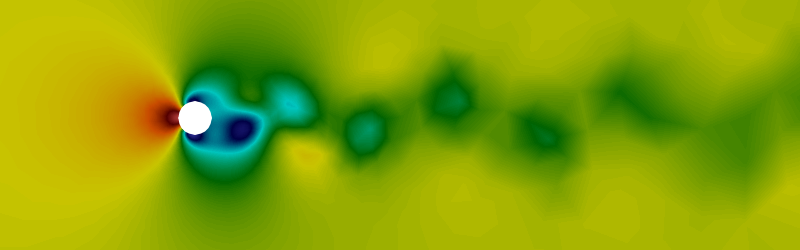
\includegraphics[width=\linewidth]{Figuras/cylinder/analise2/none-TH-p.png}
        \end{subfigure}
        \caption{Sem modelo}
    \end{subfigure}
    \begin{subfigure}{\textwidth}\centering
        \begin{subfigure}{.49\textwidth}
            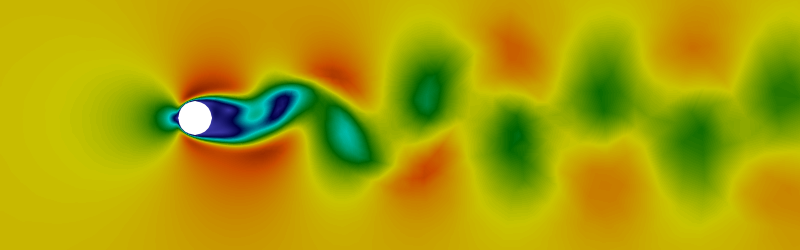
\includegraphics[width=\linewidth]{Figuras/cylinder/analise2/LES-TH-u.png}
        \end{subfigure}
        \begin{subfigure}{.49\textwidth}
            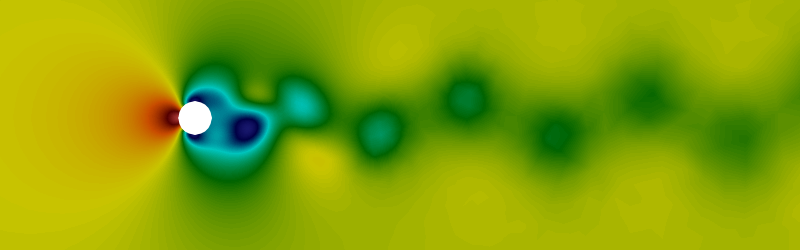
\includegraphics[width=\linewidth]{Figuras/cylinder/analise2/LES-TH-p.png}
        \end{subfigure}
        \caption{LES}
    \end{subfigure}
    \begin{subfigure}{\textwidth}\centering
        \begin{subfigure}{.49\textwidth}
            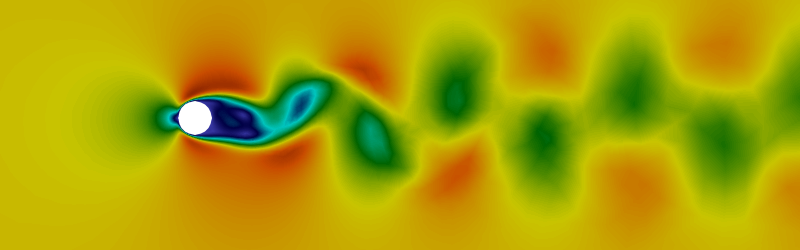
\includegraphics[width=\linewidth]{Figuras/cylinder/analise2/VMS-TH-u.png}
        \end{subfigure}
        \begin{subfigure}{.49\textwidth}
            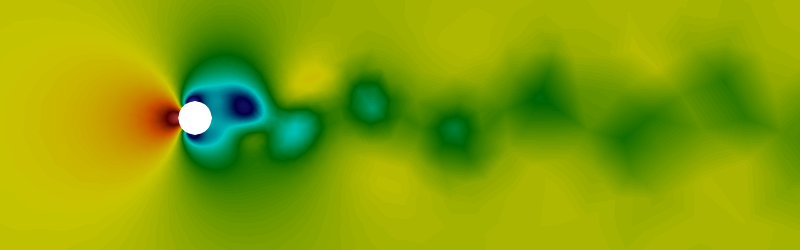
\includegraphics[width=\linewidth]{Figuras/cylinder/analise2/VMS-TH-p.png}
        \end{subfigure}
        \caption{VMS}
    \end{subfigure}
    \\Fonte: Autoria Própria (\the\year).
    \label{fig:vel-pre-TH}
\end{figure}